\documentclass[11pt,a4paper]{article}
\usepackage[utf8]{inputenc}
\usepackage[T1]{fontenc}
\usepackage[spanish,es-tabla]{babel}
\usepackage[margin=1.8cm, top=1.9cm, bottom=1.9cm]{geometry}
\setlength{\headheight}{21.3pt} % Ajusta la altura del encabezado según la sugerencia
\addtolength{\topmargin}{-9.3pt} % Compensa el margen superior para no mover el texto hacia abajo
\usepackage{graphicx}
\usepackage{booktabs}
\usepackage{amsmath,amssymb}
\usepackage{tabularx}
\usepackage{xcolor}
\usepackage{titlesec}
\usepackage{enumitem}
\usepackage[hyphens]{url}
\usepackage{hyperref}
\urlstyle{same}
\usepackage{fancyhdr}
\usepackage{caption}
\usepackage{subcaption}
\usepackage{float}
\usepackage{parskip}
\usepackage{multicol}
\usepackage{setspace}
\usepackage{array}
\usepackage{multirow}
\usepackage{colortbl}
\usepackage{tcolorbox}

\tcbuselibrary{skins}

% ── PALETA ──────────────────────────────────────────────────
\definecolor{azuloscuro}{HTML}{1F4E79}
\definecolor{azulclaro}{HTML}{2E75B6}
\definecolor{grisclaro}{HTML}{F2F7FB}
\definecolor{grismedio}{HTML}{A8A7A7}
\definecolor{rojosuave}{HTML}{C0392B}
\definecolor{verdeclaro}{HTML}{1E6B3C}
\definecolor{verdesuave}{HTML}{D9EAD3}
\definecolor{naranjaalerta}{HTML}{FCE4D6}
\definecolor{azulsuave}{HTML}{E7F0F9}

\hypersetup{colorlinks=true,linkcolor=azuloscuro,urlcolor=azulclaro,citecolor=azuloscuro}
\titleformat{\section}{\normalsize\bfseries\color{azuloscuro}}{\thesection.}{0.5em}{}[\vspace{-0.3em}]
\titleformat{\subsection}{\small\bfseries\color{azulclaro}}{\thesubsection.}{0.5em}{}[\vspace{-0.2em}]
\titleformat{\subsubsection}{\small\bfseries\color{azulclaro!80!black}}{\thesubsubsection.}{0.4em}{}[\vspace{-0.15em}]
\titlespacing*{\section}{0pt}{0.6em}{0.15em}
\titlespacing*{\subsection}{0pt}{0.4em}{0.1em}
\titlespacing*{\subsubsection}{0pt}{0.3em}{0.08em}

\pagestyle{fancy}
\fancyhf{}
\fancyhead[L]{\footnotesize\textcolor{azuloscuro}{Optimización del Portafolio de Importaciones de Bogotá}}
\fancyhead[R]{\footnotesize\textcolor{azuloscuro}{\thepage/10}}
\renewcommand{\headrulewidth}{0.4pt}
\renewcommand{\headrule}{\hbox to\headwidth{\color{azuloscuro}\leaders\hrule height \headrulewidth\hfill}}

\setlength{\parskip}{0.2em}
\setlength{\parindent}{0pt}
\captionsetup{font=footnotesize,labelfont=bf,skip=2pt}
\setstretch{1.0}

\newtcolorbox{hallazgo}{colback=grisclaro,colframe=azuloscuro,arc=1mm,boxrule=0.4pt,
    left=2mm,right=2mm,top=1mm,bottom=1mm,fontupper=\footnotesize}
\newtcolorbox{recomendacion}{colback=verdesuave,colframe=verdeclaro,arc=1mm,boxrule=0.5pt,
    left=2mm,right=2mm,top=1mm,bottom=1mm,fontupper=\footnotesize}
\newtcolorbox{insight}{colback=azulsuave,colframe=azulclaro,arc=1mm,boxrule=0.4pt,
    left=2mm,right=2mm,top=1mm,bottom=1mm,fontupper=\footnotesize}

\title{\vspace{-1.8cm}
    \textcolor{azuloscuro}{\textbf{\Large Optimización del Portafolio de Importaciones de Bogotá}} \\[0.1cm]
    \normalsize\textcolor{azulclaro}{\textit{Modelo integrado basado en datos para la toma de decisiones organizacionales}}}
\author{\small Johan Nicolás Valderrama Serrato \quad Mariana Prada Riaño \quad Paola Andrea Castro \\[0.05cm]
\footnotesize\textit{Toma de Decisiones Organizacionales}}
\date{\footnotesize\today}

\begin{document}
\maketitle
\thispagestyle{fancy}
\vspace{-1cm}

% ==========================================================================
\section{Introducción}
% ==========================================================================

\subsection{Descripción del problema y contexto}

Bogotá es el principal hub de importaciones de Colombia. Durante enero--julio 2025, la ciudad registró importaciones por USD 39.998M CIF provenientes de 189 países, según 238.305 registros obtenidos del Portal de Datos Abiertos de Bogotá. Sin embargo, solo dos países (China con 26.5\% y Estados Unidos con 24.3\%) concentran el 51\% del valor total, exponiendo la cadena de suministro a riesgos geopolíticos (guerra comercial EE.UU.--China), logísticos (congestión portuaria, pandemias, conflictos regionales) y arancelarios. La severidad del problema se amplifica porque el 48.5\% de las importaciones son materias primas que alimentan cadenas productivas completas: una disrupción de suministro no solo afecta al importador directo, sino que paraliza sectores enteros (manufactura, construcción, agroindustria).

\subsection{Objetivo de la decisión}

Determinar la asignación óptima de participaciones por país en el portafolio de importaciones de Bogotá que minimice el costo logístico total más el costo de transición respecto al portafolio actual, sujeto a: un presupuesto de riesgo geopolítico acotado, cumplimiento de política comercial (mínimo 40\% desde países con TLC), restricciones anti-concentración (ningún país $>$ 25\%) y  participación mínima por país ($\geq$ 0.5\%) para mantener relaciones comerciales.

\subsection{Justificación del enfoque data-driven}

El volumen de datos (238.305 registros con 17 columnas analíticas: país, partida arancelaria, uso económico, nivel tecnológico, valor CIF/FOB, peso) justifica un enfoque cuantitativo. La intuición directiva, sin modelo formal, pasa por alto trade-offs no evidentes: los países más seguros (Francia, Alemania) son también los más baratos logísticamente, hallazgo contraintuitivo que solo emerge al integrar optimización matemática con análisis de sensibilidad y validación estocástica.

\subsection{Delimitación}

\textbf{Temporalidad:} enero--julio 2025 (7 meses de datos reales, sin datos sintéticos). \textbf{Granularidad:} país de origen como unidad de decisión. \textbf{Impacto:} USD 35.244M en decisiones de compra (89.6\% del CIF total, correspondiente al cluster estratégico). \textbf{Acceso a datos:} API pública CKAN del Portal de Datos Abiertos. \textbf{Enfoque:} estático sobre el portafolio agregado, con análisis dinámico vía simulación. \textbf{Herramientas (3):} Python (PuLP, scikit-learn, NumPy, SciPy, matplotlib)

% ==========================================================================
\section{Metodología}
% ==========================================================================

El proyecto integra análisis cualitativo y cuantitativo complejo: analítica descriptiva + optimización lineal + simulación estocástica. Cada etapa alimenta los parámetros de la siguiente, cerrando un circuito coherente entre juicio experto y formulación matemática.

\subsection{Análisis cualitativo}

\subsubsection{Componente observacional}

Se construyó una matriz estructurada de cinco hallazgos observacionales (hallazgo --causa --riesgo --implicación) derivados del EDA y literatura en supply chain risk management: (i) concentración 51\% en dos países $\Rightarrow$ riesgo sistémico $\Rightarrow$ restricción $\bar{x}$; (ii) 48.5\% materias primas $\Rightarrow$ parálisis de cadenas productivas $\Rightarrow$ alto peso al riesgo geopolítico; (iii) heterogeneidad CIF/FOB 1.00--1.39 $\Rightarrow$ sobrecostos ocultos $\Rightarrow$ objetivo de minimización; (iv) sub-uso de TLC $\Rightarrow$ pago innecesario de aranceles $\Rightarrow$ restricción $L_{TLC}$; (v) número efectivo de proveedores $N_{eff} \approx 7.2$ (vs. 189 nominales) $\Rightarrow$ diversidad engañosa $\Rightarrow$ objetivo real: reducir HHI del cluster.

\subsubsection{Modelo cualitativo formal: AHP}

Proceso Analítico Jerárquico (Saaty, 1980) sobre cinco criterios: costo CIF, diversificación, confiabilidad logística, nivel tecnológico y riesgo geopolítico. La matriz de comparaciones pareadas se construyó fundamentada en literatura: Chopra \& Sodhi (2014) para la preeminencia de la diversificación; Christopher \& Peck (2004) para la resiliencia estructural; Manuj \& Mentzer (2008) para la subordinación del nivel tecnológico. Pesos obtenidos por el método del autovector principal con CR = 0.0074 ($<$ 0.10, consistente). Los pesos AHP por criterio informan cualitativamente el diseño del modelo LP: el peso dominante de la diversificación (40.3\%) justifica incluir el presupuesto de riesgo R3 como restricción y no como término en la función objetivo.

\subsection{Análisis cuantitativo complejo}

\subsubsection{Analítica descriptiva y clustering K-Means}

Métricas de concentración: HHI global y mensual, coeficiente de Gini, curva de Lorenz, análisis Pareto y número efectivo de proveedores $N_{eff} = 1/\sum p_i^2$. Se analizaron composición por uso económico, nivel tecnológico y mapa bidimensional de eficiencia logística. Para la segmentación, se aplicó K-Means sobre 67 países relevantes usando cuatro features transformadas logarítmicamente:
$$
\{\text{CIF/FOB},\ \log(\text{precio/kg}),\ \log(\text{CIF}),\ \log(\text{n\_transacciones})\}
$$
Selección $k=4$ validada con \textit{silhouette score} = 0.355; visualización con reducción PCA a 2D y panel de \emph{loadings} interpretable.

\subsubsection{Modelo de programación lineal con presupuesto de riesgo}

\textbf{Planteamiento.} El cluster ``Socios Estratégicos'' identificado por K-Means contiene 24 países y concentra el 89.6\% del CIF. Tras excluir metodológicamente a Colombia (Zona Franca) por ser territorio aduanero nacional, el modelo LP opera sobre \textbf{$|I|=23$ países} con demanda agregada de \textbf{USD 35.244M}.

\vspace{0.1cm}
\noindent\textbf{Conjuntos e índices:}
\vspace{-0.1cm}
\begin{itemize}[noitemsep,topsep=0pt,leftmargin=1.3em]
\footnotesize
\item $I$: países proveedores del cluster estratégico ($|I| = 23$).
\item $T \subseteq I$: países con TLC vigente con Colombia ($|T| = 13$).
\end{itemize}

\vspace{0.1cm}
\noindent\textbf{Parámetros:}
\vspace{-0.1cm}
\begin{itemize}[noitemsep,topsep=0pt,leftmargin=1.3em]
\footnotesize
\item $c_i$: costo logístico unitario (ratio CIF/FOB observado). Mide el sobrecosto de flete + seguro por cada USD de valor FOB (p.ej. $c_{\text{Francia}}=1.033$, $c_{\text{China}}=1.068$).
\item $r_i$: score de riesgo geopolítico (escala 0--10), \emph{calibrado} con el Global Risk Index 2024 (WEF) y el Economic Complexity Index (Harvard). P.ej. $r_{\text{China}}=8.5$, $r_{\text{Francia}}=3.0$.
\item $a_i$: participación actual (observada enero--julio 2025).
\item $\tau = 0.048$: costo de transición por unidad de cambio, calibrado al rango de $c_i$ para evitar saltos extremos.
\item $R_{max}$: presupuesto máximo de riesgo ponderado (parámetro de política).
\item $\underline{x}=0.005$: participación mínima por país (evita exclusión total).
\item $\bar{x}=0.25$: participación máxima por país (política anti-concentración).
\item $L_{TLC}=0.40$: mínimo desde socios con TLC (aprovecha preferencias arancelarias).
\end{itemize}

\vspace{0.1cm}
\noindent\textbf{Variables de decisión:}
\vspace{-0.1cm}
\begin{itemize}[noitemsep,topsep=0pt,leftmargin=1.3em]
\footnotesize
\item $x_i \geq 0$: proporción del cluster asignada al país $i$ ---\emph{la incógnita principal}.
\item $\delta_i^+ \geq 0$: incremento de $x_i$ respecto a $a_i$.
\item $\delta_i^- \geq 0$: reducción de $x_i$ respecto a $a_i$.
\end{itemize}

\vspace{0.1cm}
\noindent\textbf{Función objetivo:}
\vspace{-0.1cm}
\begin{equation}
\boxed{\ \min\ Z = \underbrace{\sum_{i \in I} c_i \cdot x_i}_{\substack{\text{costo logístico} \\ \text{ponderado (recurrente)}}} \ +\ \underbrace{\tau \cdot \sum_{i \in I} \left(\delta_i^+ + \delta_i^-\right)}_{\substack{\text{costo de transición} \\ \text{(único, por cambio)}}} \ }
\label{eq:fo}
\end{equation}

El primer término minimiza el costo logístico del portafolio (gasto recurrente en flete + seguro). El segundo término penaliza los cambios respecto al portafolio actual, representando costos reales de renegociación de contratos, certificaciones y adecuación logística. Evita soluciones que reorganicen el portafolio drásticamente sin justificación económica.

\vspace{0.1cm}
\noindent\textbf{Restricciones:}
\vspace{-0.1cm}
\begin{align}
\sum_{\forall i \in I} x_i &= 1 
& &\text{(R1 --- Asignación completa)} \label{eq:r1}\\
x_i - a_i &= \delta_i^+ - \delta_i^- 
& &\forall i \in I \quad \text{(R2 --- Balance de transición)} \label{eq:r2}\\
\sum_{\forall i \in I} r_i \cdot x_i &\leq R_{max} 
& &\text{(R3 --- Presupuesto de riesgo)} \label{eq:r3}\\
\sum_{\forall i \in T} x_i &\geq L_{TLC} 
& &\text{(R4 --- Política comercial TLC)} \label{eq:r4}\\
\underline{x} \leq x_i &\leq \bar{x} 
& &\forall i \in I \quad \text{(R5 --- Cotas por país)} \label{eq:r5}\\
x_i,\ \delta_i^+,\ \delta_i^- &\geq 0 
& &\forall i \in I \quad \text{(R6 --- No negatividad)} \label{eq:r6}
\end{align}

La restricción R3 es la decisión de diseño central: convierte el riesgo geopolítico en una restricción dura infranqueable, garantizando que cualquier óptimo cumpla la meta estratégica de reducción sin depender de pesos subjetivos en la F.O.

\subsubsection{Análisis de escenarios de política de riesgo}

Se definieron tres configuraciones discretas del parámetro $R_{max}$ que representan distintas posturas de política, resolviendo un LP independiente por cada una: \textbf{Permisivo} ($R_{max} = R_{actual} = 5.684$; mantiene el nivel de riesgo actual), \textbf{Moderado} ($R_{max} = 0.85\, R_{actual} = 4.831$; reduce 15\%, recomendado) y \textbf{Estricto} ($R_{max} = 0.70\, R_{actual} = 3.979$; reduce 30\%).

\subsubsection{Análisis de sensibilidad (dual y paramétrico)}

Complementa al análisis de escenarios. Se explotó la solución dual del LP del escenario Moderado para identificar: restricciones activas (con holgura cero, que ``atan'' el óptimo), precios sombra $\pi_k$ (tasa de cambio marginal de $Z^*$ al aumentar el lado derecho de la restricción $k$ en una unidad, costos reducidos (países en cotas vs. en región interior). Adicionalmente, se realizó un análisis de sensibilidad: el LP se resolvió 25 veces con $R_{max}$ variando en $[0.50, 1.10]\cdot R_{actual}$, trazando la curva completa $Z^*(R_{max})$ y HHI$(R_{max})$.

\subsubsection{Simulación Monte Carlo}

Evalúa la robustez del portafolio óptimo $x_i^*$ (escenario Moderado) ante incertidumbre estocástica en 10.000 iteraciones. El costo total en cada iteración $n$ se modela:
\vspace{-0.1cm}
\begin{equation}
\text{Costo}_n = \underbrace{\sum_{i \in I} c_i \cdot x_i^* \cdot D \cdot S_i^{(n)} \cdot \text{FX}^{(n)} \cdot \epsilon_i^{(n)}}_{\text{costo de importación efectiva}} + \underbrace{\phi \cdot D \cdot \text{FX}^{(n)} \cdot \left(1 - \sum_{i} x_i^* \cdot S_i^{(n)}\right)^+}_{\text{penalidad por faltante (compra spot)}}
\label{eq:mc}
\end{equation}
donde $D=$ USD 35.244M, $(z)^+=\max(0,z)$ y $\phi=1.5$ (sobrecosto del 50\% por compras de emergencia).

\begin{table}[H]
\centering\caption{Variables estocásticas de la simulación Monte Carlo}\label{tab:vars_mc}
\footnotesize
\begin{tabularx}{\textwidth}{lcX}
\toprule
\textbf{Variable} & \textbf{Distribución} & \textbf{Justificación} \\
\midrule
$\text{FX}^{(n)}$ (tipo de cambio) & $\mathcal{N}(1.0,\ 0.05)$ & Volatilidad mensual USD/COP observada ($\pm 5\%$) \\
$S_i^{(n)}$ (factor de suministro) & Bernoulli($p_i$) & $p_i$ por nivel de riesgo: 12\% alto, 5\% medio, 3\% con TLC \\
Magnitud disrupción & $\mathcal{U}(0.20, 0.80)$ & Reducción de capacidad condicional a disrupción \\
$\epsilon_i^{(n)}$ (shock logístico) & $\text{LogNormal}(0, 0.08)$ & Asimetría: los fletes suben más fácilmente que bajan \\
\bottomrule
\end{tabularx}
\end{table}

\vspace{-0.3cm}
\textbf{Escenarios Monte Carlo} (comparación simétrica Base vs. Óptimo con misma semilla e idénticos shocks): (1) Normal: disrupciones con probabilidades $p_i$ por nivel de riesgo; (2) Estrés China $-50\%$: disrupción severa en China ($S_{\text{China}}^{(n)}=0.5$ en todas las iteraciones); (3) Estrés dual: disrupción simultánea en China y EE.UU. Estos escenarios Monte Carlo (estocásticos, sobre el portafolio) se diferencian de los escenarios de política (deterministas, sobre $R_{max}$).

\subsection{Validación: KPIs y KPPs}

Tablero con: HHI, participación Top 5, costo logístico ponderado (CIF/FOB), riesgo ponderado, VaR y CVaR 95\%, cobertura media de demanda, P(cobertura $<$ 90\%) como probabilidad de falla crítica, y número de países activos.

% ==========================================================================
\section{Resultados}
% ==========================================================================

\subsection{Diagnóstico: concentración estructural}

El portafolio global de Bogotá presenta HHI = 1.397, lo que según la clasificación del DOJ/FTC (2023) corresponde a un mercado no concentrado ($<$ 1.500), solo marginalmente por debajo del umbral de concentración moderada. No obstante, al analizar exclusivamente el cluster estratégico (donde reside el 89.6\% del valor), el HHI sube a 1.790, ubicándose en el rango moderadamente concentrado (1.500--2.500). La Figura~\ref{fig:concentracion} muestra tres dimensiones complementarias del diagnóstico.

\begin{figure}[H]
\centering
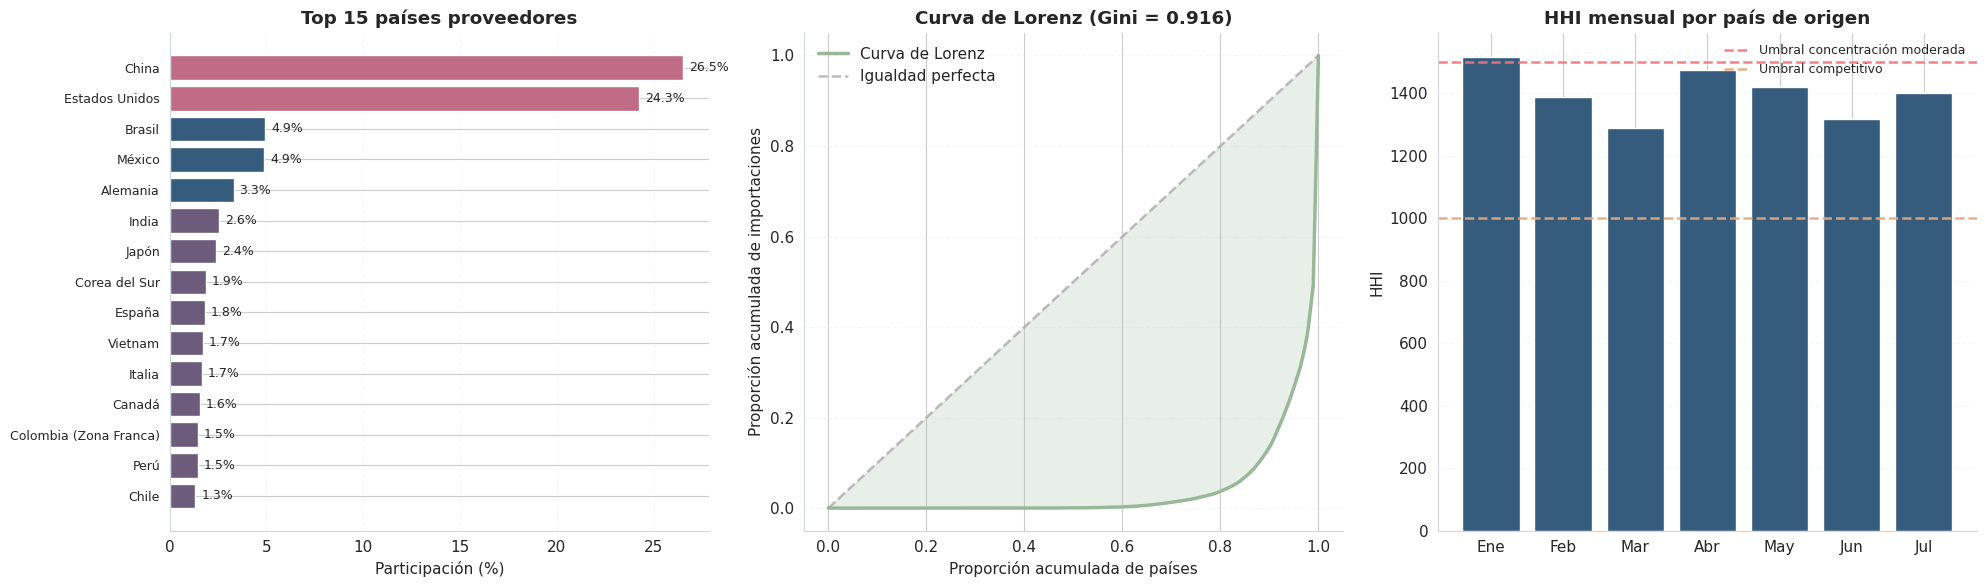
\includegraphics[width=0.96\textwidth]{distribucion_paises.png}
\caption{\textbf{Análisis integral de concentración.} (Izq.) Top 15 países: China (26.5\%) y EE.UU. (24.3\%) dominan más del doble que Brasil (4.9\%). (Centro) Curva de Lorenz con Gini=0.916 $\Rightarrow$ desigualdad extrema: el 90\% de los países aporta menos del 20\% del valor. (Der.) HHI mensual en banda estable 1.300--1.500 $\Rightarrow$ concentración \emph{estructural}, no coyuntural.}
\label{fig:concentracion}
\end{figure}

\vspace{-0.3cm}
\begin{hallazgo}
\textbf{Hallazgo 1 --- Diversidad engañosa:} con $N_{eff}\approx 7.2$, los 189 países nominales equivalen efectivamente a menos de 8 proveedores homogéneos.
\end{hallazgo}

El mapa de eficiencia logística (Figura~\ref{fig:logistica}) revela el hallazgo que hace posible la solución: Francia (1.033), Alemania (1.034) y Ecuador (1.032) tienen ratios CIF/FOB menores que China (1.068) y Brasil (1.069). La concentración actual no es el resultado de una optimización económica, sino de inercia histórica comercial.

\begin{figure}[H]
\centering
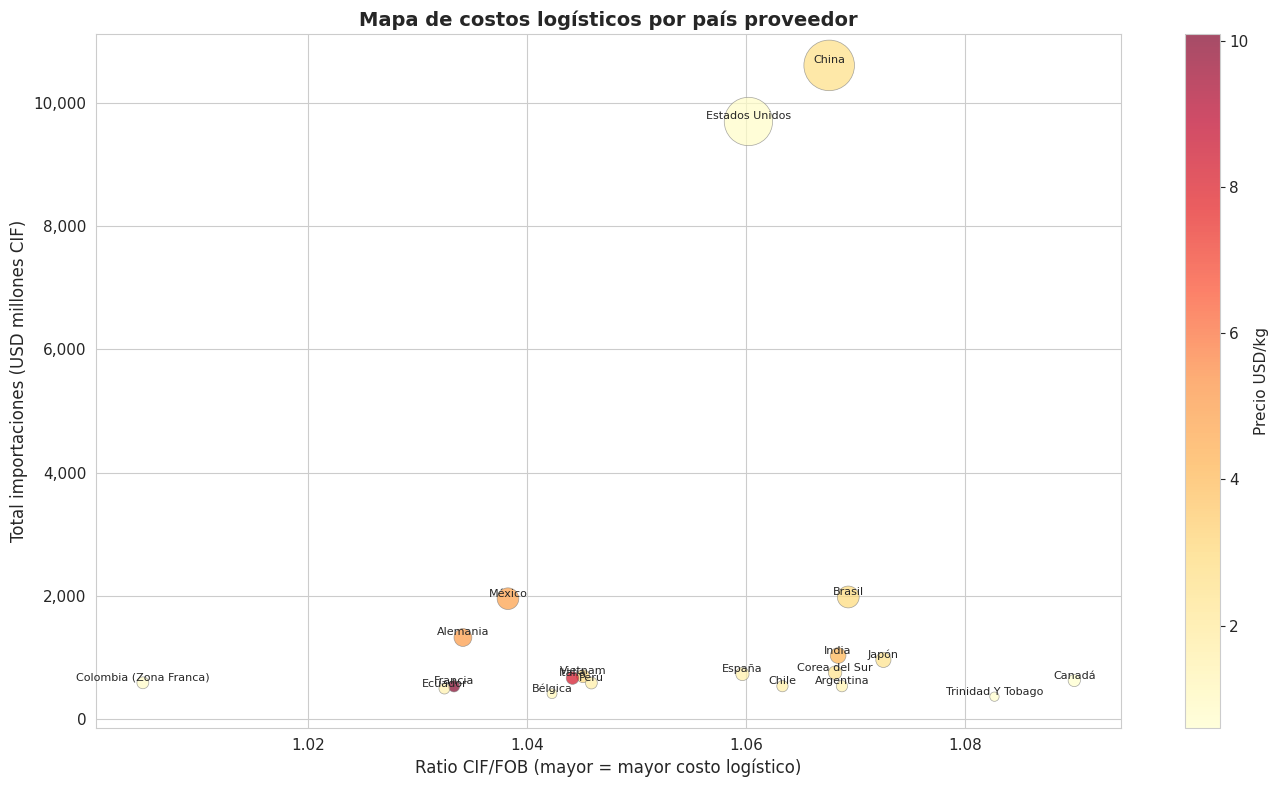
\includegraphics[width=0.68\textwidth]{mapa_costos_logisticos.png}
\caption{\textbf{Mapa de costos logísticos por país.} Eje X: ratio CIF/FOB; eje Y: volumen CIF; color: precio USD/kg. China y EE.UU. (burbujas mayores) tienen ratios \emph{superiores} a Francia, Alemania y Ecuador (esquina inferior izquierda, cuadrante óptimo). \textbf{Hallazgo crucial: diversificar no es más caro.}}
\label{fig:logistica}
\end{figure}

\vspace{-0.3cm}
\subsection{AHP y segmentación por K-Means}

El AHP (CR=0.0074, consistente) prioriza diversificación (40.3\%) sobre costo (24.4\%), confiabilidad (13.7\%), riesgo geopolítico (13.7\%) y tecnología (7.9\%). La dominancia de la diversificación motiva incluir $R_{max}$ como restricción dura en lugar de como término ponderado en la F.O. (Figura~\ref{fig:ahp}).

\begin{figure}[H]
\centering
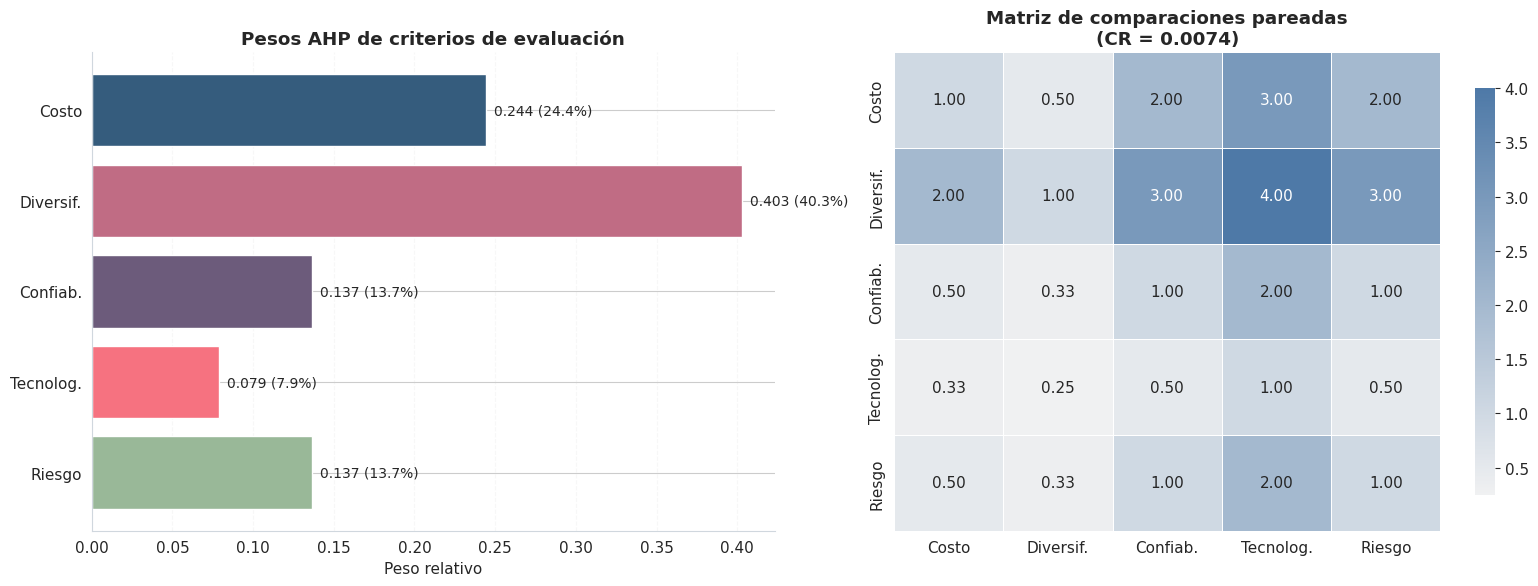
\includegraphics[width=0.92\textwidth]{pesos_ahp.png}
\caption{\textbf{AHP --- priorización de criterios.} (Izq.) Pesos normalizados: \emph{diversificación} domina (40.3\%), consistente con literatura en entornos de alta incertidumbre geopolítica. (Der.) Matriz de comparaciones pareadas escala Saaty 1--9 con CR=0.0074 $\Rightarrow$ juicios consistentes.}
\label{fig:ahp}
\end{figure}

\vspace{-0.3cm}
K-Means ($k=4$, silhouette=0.355) produce cuatro perfiles. El Cluster 0 identificado por el algoritmo contiene 24 países y concentra el 89.6\% del CIF; tras excluir Colombia (Zona Franca), el modelo LP opera sobre 23 países internacionales (Cuadro~\ref{tab:clusters}, Figura~\ref{fig:clusters}).

\begin{table}[H]
\centering\caption{Perfiles de los cuatro clusters identificados por K-Means}\label{tab:clusters}
\footnotesize
\begin{tabularx}{\textwidth}{clccclX} % Añadimos X al final para que sea flexible
\toprule
\textbf{C} & \textbf{Nombre} & \textbf{Países} & \textbf{\% CIF} & \textbf{CIF/FOB} & \textbf{Representantes} \\
\midrule
\rowcolor{verdesuave}
\textbf{0} & \textbf{Socios Estratégicos} & \textbf{24}$^{*}$ & \textbf{89.6\%} & 1.056 & China, EE.UU., Brasil, México, Alemania \\
1 & Proveedores Eficientes & 25 & 5.8\% & 1.042 & Suiza, Reino Unido, Irlanda, Suecia \\
2 & Prov. Ocasionales & 17 & 4.0\% & 1.075 & Trinidad, Rusia, Bolivia, Finlandia \\
3 & Proveedor Atípico & 1 & 0.1\% & 1.388 & Argelia \\
\bottomrule
\multicolumn{6}{l}{\footnotesize $^{*}$El modelo LP opera sobre 23 países tras excluir Colombia (Zona Franca).}
\end{tabularx}
\end{table}

\vspace{-0.3cm}
\begin{figure}[H]
\centering
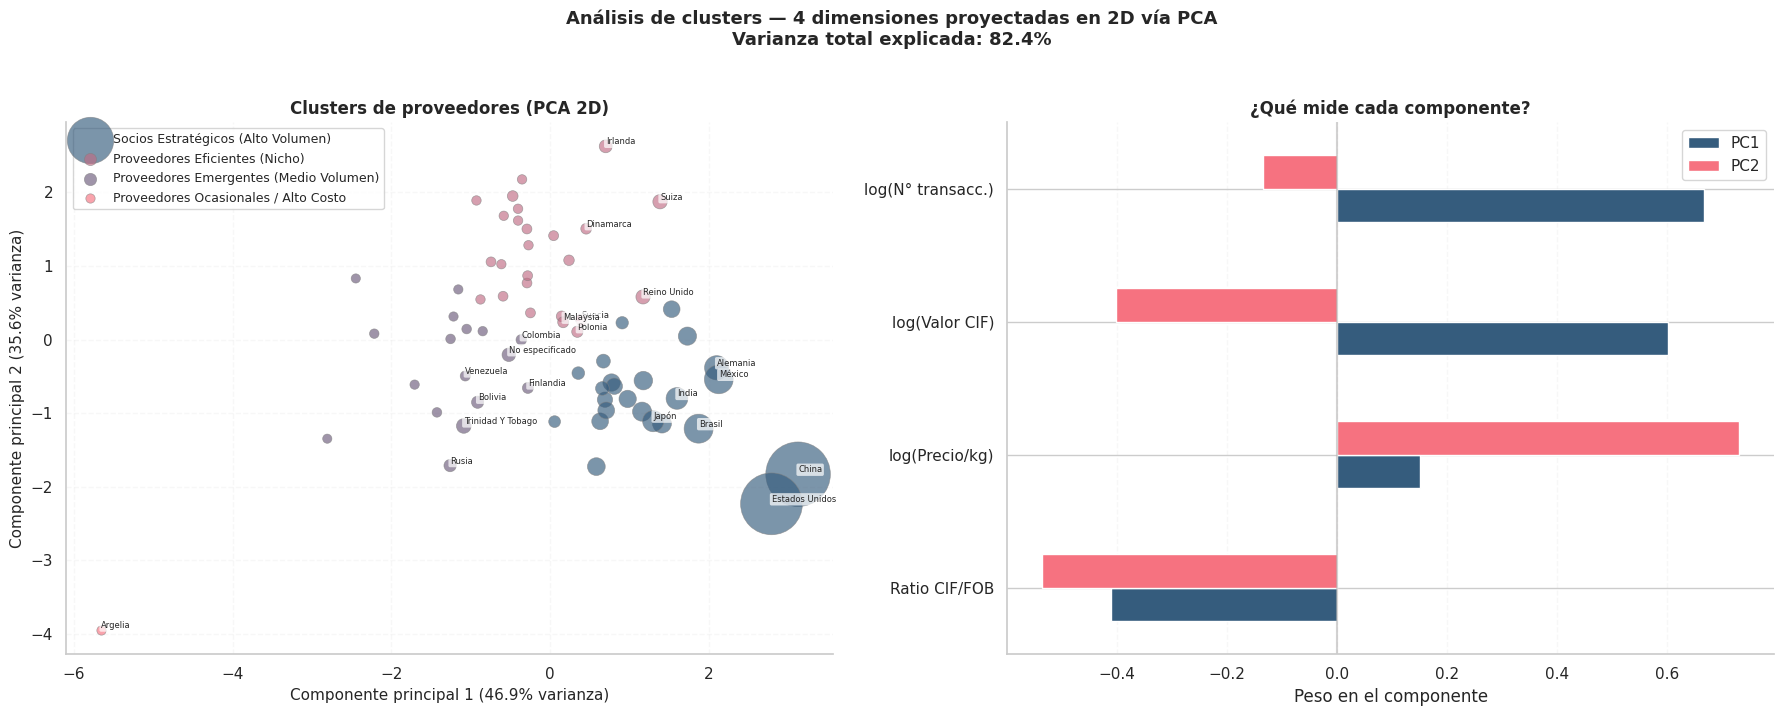
\includegraphics[width=0.96\textwidth]{analisis_cluster.png}
\caption{\textbf{Clusters en espacio PCA 2D} (82.4\% varianza explicada). (Izq.) Cuatro perfiles separados; China y EE.UU. son outliers de volumen; Argelia es caso atípico aislado. (Der.) \emph{Loadings}: PC1 mide volumen comercial (log CIF, log transacciones); PC2 mide perfil logístico (ratio CIF/FOB, precio/kg).}
\label{fig:clusters}
\end{figure}

\vspace{-0.3cm}
\subsection{Resultado del LP bajo escenario Moderado}

El solver CBC resolvió óptimamente el LP (estado: \emph{Optimal}). El Cuadro~\ref{tab:resultados_opt} presenta los KPIs: la redistribución mejora el costo logístico recurrente, el riesgo geopolítico y la concentración HHI \emph{simultáneamente}; el único KPI que empeora es el costo total de la F.O., exclusivamente por el término \emph{único} de transición.

\begin{table}[H]
\centering\caption{KPIs del modelo LP (escenario Moderado, $R_{max}=0.85\cdot R_{actual}$)}\label{tab:resultados_opt}
\footnotesize
\begin{tabularx}{\textwidth}{Xcccc}
\toprule
\textbf{Métrica (KPI)} & \textbf{Base} & \textbf{Óptimo} & \textbf{$\Delta$} & \textbf{Evaluación} \\
\midrule
Costo logístico $Z$ (CIF/FOB ponderado)         & 1.0604 & 1.0548 & $-0.53\%$ & \textcolor{verdeclaro}{\checkmark\ Menor que actual} \\
Costo de transición $\tau\sum(\delta^++\delta^-)$ & ---    & 0.0164 & ---         & Costo único, no recurrente \\
Costo total F.O. (incl. transición)             & 1.0604 & 1.0712 & $+1.02\%$ & Trade-off aceptado por resiliencia \\
Riesgo geopolítico ponderado                    & 5.684  & 4.831  & $-15.00\%$ & \textcolor{verdeclaro}{\checkmark\ Meta cumplida} \\
HHI del cluster                                 & 1.790  & 1.335  & $-25.4\%$ & \textcolor{verdeclaro}{\checkmark\ Reducción significativa} \\
Máx. participación por país                     & 30.1\% & 25.0\% & $-5.1$ p.p. & \textcolor{verdeclaro}{\checkmark\ Cumple $\bar{x}$} \\
Participación desde TLC                         & 62\%   & 62\%   & 0           & Por encima del 40\% exigido \\
\bottomrule
\end{tabularx}
\end{table}

\vspace{-0.3cm}
\textbf{Interpretación económica de los movimientos.} La solución es un vértice no degenerado: de las 26 restricciones del modelo, 25 son activas (R1, R2 para los 23 países, R3 y una de las cotas en R5 para EE.UU.), lo que explica por qué solo tres países cambian significativamente:
\vspace{-0.1cm}
\begin{itemize}[noitemsep,topsep=0pt,leftmargin=1.3em]
\footnotesize
\item \textbf{Francia (1.50\% $\to$ 18.59\%, +17.09 p.p.):} alternativa dominante a China por triple razón: más barata ($c=1.033$ vs. $c_{\text{China}}=1.068$), más segura ($r=3.0$ vs. $r_{\text{China}}=8.5$) y con TLC (contribuye a R4).
\item \textbf{China (30.11\% $\to$ 15.50\%, $-$14.61 p.p.):} reducción forzada por dos motivos: violaba el techo $\bar{x}=25\%$ en R5 y tiene el mayor $r_i$ del cluster (8.5).
\item \textbf{EE.UU. (27.52\% $\to$ 25.00\%, $-$2.52 p.p.):} ajuste exacto al techo $\bar{x}=25\%$; el modelo prefiere mantenerlo en el máximo por su TLC y menor $r_i$ que China.
\item \textbf{20 países restantes:} mantienen su participación actual. Al operar con R3 activa, la asignación queda determinada por el vértice del poliedro factible.
\end{itemize}

\begin{hallazgo}
\textbf{Hallazgo 2 --- Mejora multicriterio simultánea:} el portafolio óptimo reduce costo logístico, riesgo y concentración al mismo tiempo. El incremento del $+1.02\%$ en costo total F.O. se debe exclusivamente al término \emph{único} de transición; el costo recurrente de operación es \emph{inferior} al actual.
\end{hallazgo}

\subsection{Análisis de sensibilidad del LP óptimo}

\subsubsection{Información dual (costo marginal de las restricciones)}

La solución dual del LP (escenario Moderado) permite cuantificar el costo marginal de cada restricción:

\textbf{Restricciones activas:} 25 de las 26 restricciones son activas (holgura cero). \textbf{R4 (TLC) es inactiva:} la suma desde países con TLC alcanza el 62\%, excediendo cómodamente el mínimo exigido de 40\%. \textbf{Precio sombra de $R_{max}$:} $\pi_{R3}=-0.0112$; relajar la restricción R3 aumentando $R_{max}$ en 0.1 unidades reduciría $Z^*$ en $\approx 0.0011$ (señal clara del costo marginal que impone la restricción de riesgo sobre la F.O.). \textbf{Países en cotas:} EE.UU. en bound máximo $\bar{x}$ (el modelo lo llevaría más arriba si pudiera); Turquía en bound mínimo $\underline{x}$ por alto $c_i=1.101$; los otros 21 países en región interior $\Rightarrow$ solución robusta, sin degeneración primal.

\subsubsection{Análisis de sensibilidad de \texorpdfstring{$R_{max}$}{Rmax}}

A diferencia del análisis de escenarios (tres configuraciones discretas de $R_{max}$; ver Sección~\ref{sec:escenarios_pol}), el análisis paramétrico barre \emph{continuamente} $R_{max}$ en $[0.50, 1.10] \cdot R_{actual}$ (25 puntos), resolviendo un LP por cada valor. La Figura~\ref{fig:sensibilidad} muestra las curvas resultantes.

\begin{figure}[H]
\centering
\begin{subfigure}{0.45\textwidth}\centering
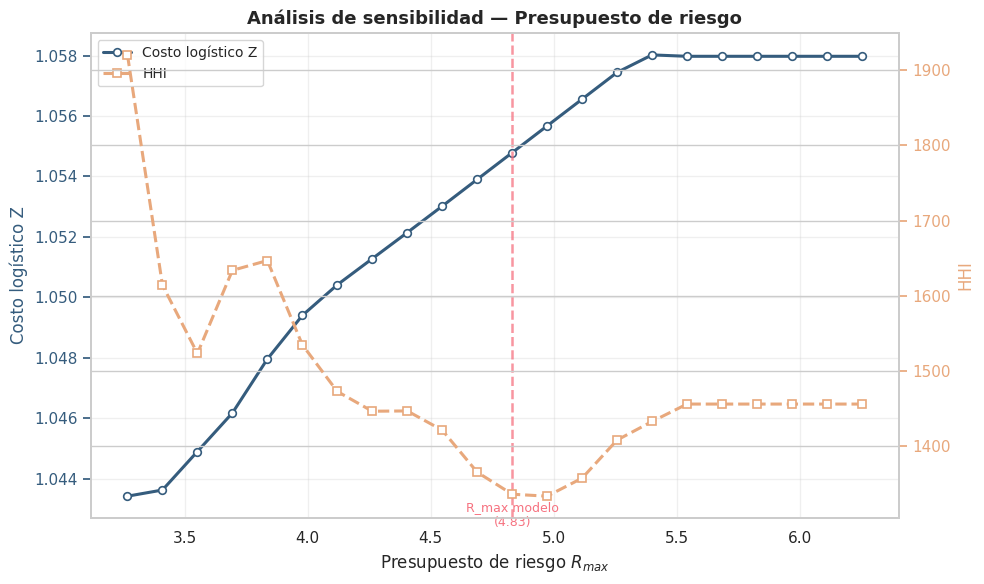
\includegraphics[width=\textwidth]{analisis_sensibilidad.png}
\caption{Curvas $Z^*$ y HHI vs. $R_{max}$}
\label{fig:sens2d}
\end{subfigure}\hfill
\begin{subfigure}{0.35\textwidth}\centering
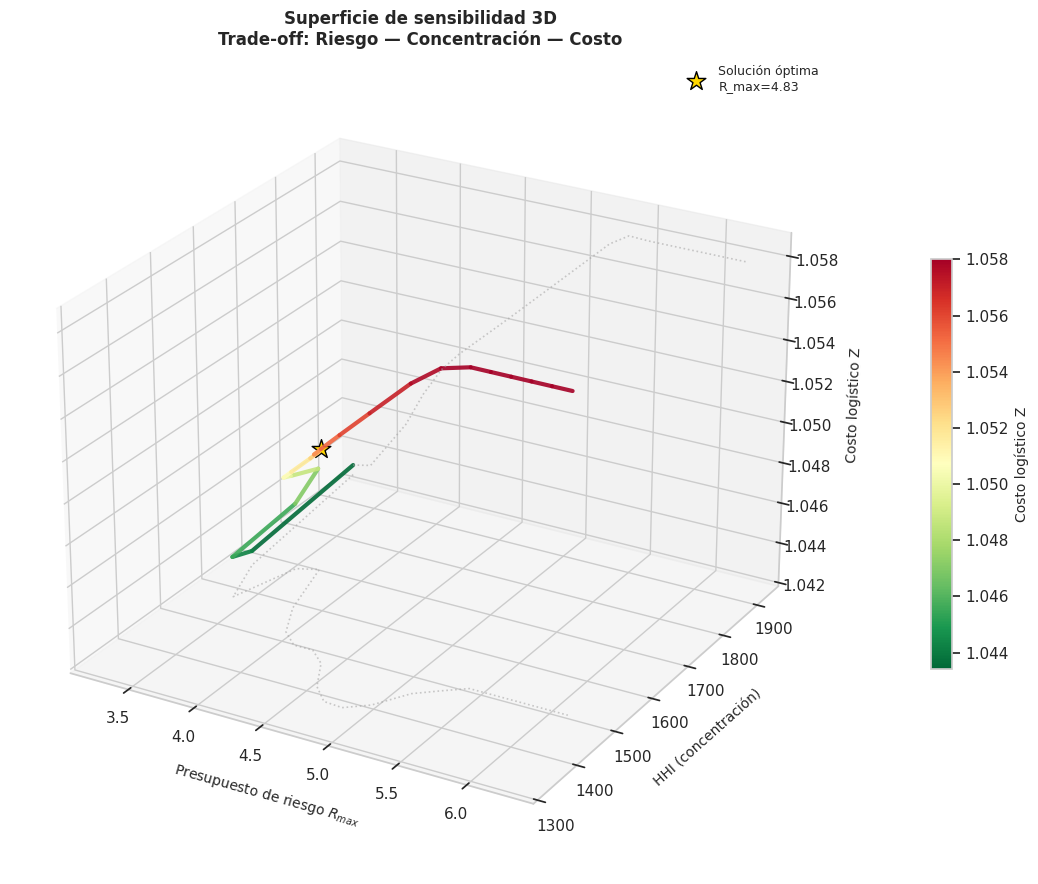
\includegraphics[width=\textwidth]{sensibilidad3d.png}
\caption{Trayectoria 3D costo--riesgo--HHI}
\label{fig:sens3d}
\end{subfigure}

\caption{\textbf{Análisis paramétrico continuo de $R_{max}$.} (a) $Z^*$ (azul) tiene pendiente positiva: al aumentar $R_{max}$ el modelo puede incluir países caros-riesgosos, elevando el costo. HHI (naranja) es no-monótono, con un mínimo local cerca de $R_{max}=4.83$. (b) Trayectoria 3D; la estrella dorada marca $R_{max}=4.83$ (escenario Moderado).}
\label{fig:sensibilidad}
\end{figure}

\vspace{-0.3cm}
\begin{insight}
\textbf{Punto de inflexión en $R_{max}\approx 3.69$.} Por debajo de este umbral, el costo marginal de reducir riesgo crece aceleradamente ---ser ultra-conservador se vuelve caro. Por encima, relajar el presupuesto no mejora significativamente el costo. El escenario Moderado ($R_{max}=4.83$) se sitúa en la región eficiente.
\end{insight}

\subsection{Análisis de escenarios de política de riesgo}
\label{sec:escenarios_pol}

A diferencia del análisis de sensibilidad (que varía un parámetro para estudiar su efecto marginal), el análisis de escenarios compara \emph{tres configuraciones discretas} de política de riesgo (Cuadro~\ref{tab:escenarios}). Cada escenario resuelve un LP independiente con su propio $R_{max}$.

\begin{table}[H]
\centering
\caption{Comparación de escenarios de política de riesgo}
\label{tab:escenarios}
\footnotesize
\begin{tabularx}{\textwidth}{lccccX} 
\toprule
\textbf{Escenario} & \textbf{$R_{max}$} & \textbf{$Z$ log.} & \textbf{$Z$ total} & \textbf{HHI} & \textbf{Evaluación} \\
\midrule
Permisivo & 5.684 & 1.0580 & 1.0653 & 1.455 & Menor costo total; reducción modesta de riesgo. \\
\rowcolor{verdesuave}
\textbf{Moderado (recomendado)} & \textbf{4.831} & \textbf{1.0548} & \textbf{1.0712} & \textbf{1.335} & \textbf{HHI mínimo; balance favorable para la toma de decisiones.} \\
Estricto & 3.979 & 1.0494 & 1.0811 & 1.534 & Menor costo logístico, pero el HHI sube por concentración en países seguros. \\
\bottomrule
\end{tabularx}
\end{table}

\vspace{-0.2cm}
El escenario \textbf{Permisivo} es informativo: aunque $R_{max} = R_{actual}$ (no exige reducción de riesgo), el LP encuentra una solución con riesgo 5.506 ($<$ 5.684) porque la cota $\bar{x}=25\%$ obliga a redistribuir China. El escenario \textbf{Estricto} presenta un resultado contraintuitivo: reducir $R_{max}$ demasiado obliga al modelo a concentrarse en los pocos países de bajo $r_i$, \emph{aumentando} el HHI (1.534 $>$ 1.455 del Permisivo). El \textbf{Moderado} ofrece el HHI mínimo dentro del rango evaluado.

\subsection{Simulación Monte Carlo: validación de robustez bajo incertidumbre}

La simulación (10.000 iteraciones, \emph{misma semilla} para Base y Óptimo $\Rightarrow$ comparación simétrica) produce las distribuciones de costo y cobertura para los cuatro casos. La Figura~\ref{fig:mc_dashboard} integra cuatro vistas.

\begin{figure}[H]
\centering
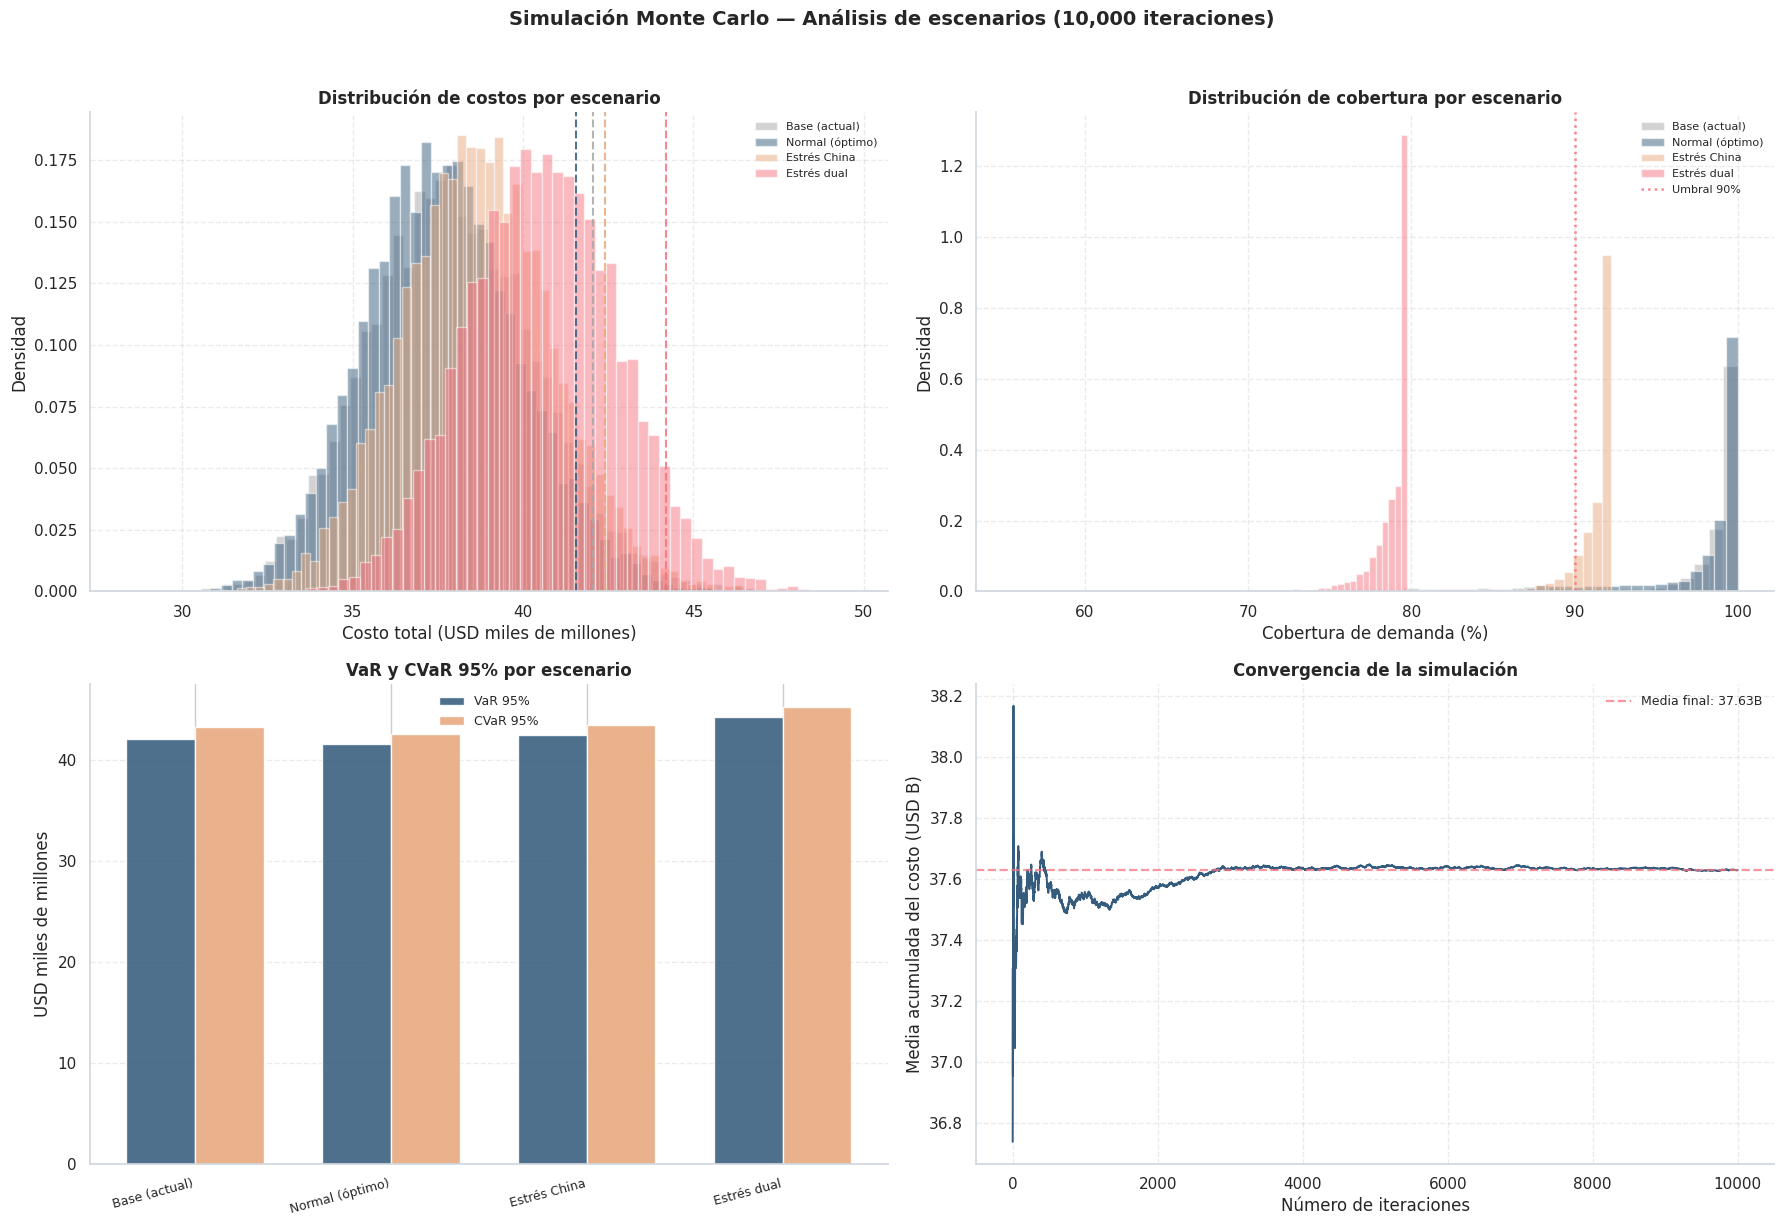
\includegraphics[width=0.98\textwidth]{resultados_montecarlo.png}
\caption{\textbf{Simulación Monte Carlo --- 10.000 iteraciones.} (Sup.~Izq.) Distribución de costos: Óptimo (azul) $<$ Base (gris) $<$ Estrés China (durazno) $<$ Estrés Dual (rosa); líneas punteadas verticales = VaR 95\%. (Sup.~Der.) Distribución de cobertura: tres \emph{modas} separadas revelan el impacto del estrés: $\sim$99\% normal, $\sim$90\% estrés China (en el umbral), $\sim$79\% estrés dual (muy bajo). (Inf.~Izq.) VaR y CVaR 95\% por escenario. (Inf.~Der.) Convergencia del costo medio: estabilización tras $\sim$2.500 iteraciones confirma suficiencia.}
\label{fig:mc_dashboard}
\end{figure}

\vspace{-0.3cm}
Los boxplots (Figura~\ref{fig:mc_boxplots}) visualizan con mayor detalle la cobertura: bajo estrés China, la caja del Base cae \emph{completamente} bajo el umbral crítico del 90\%; el Óptimo se mantiene mayoritariamente arriba. Bajo estrés dual, ambos portafolios caen bajo el 90\%: evidencia del \emph{límite estructural} del Cluster 0.

\begin{figure}[H]
\centering
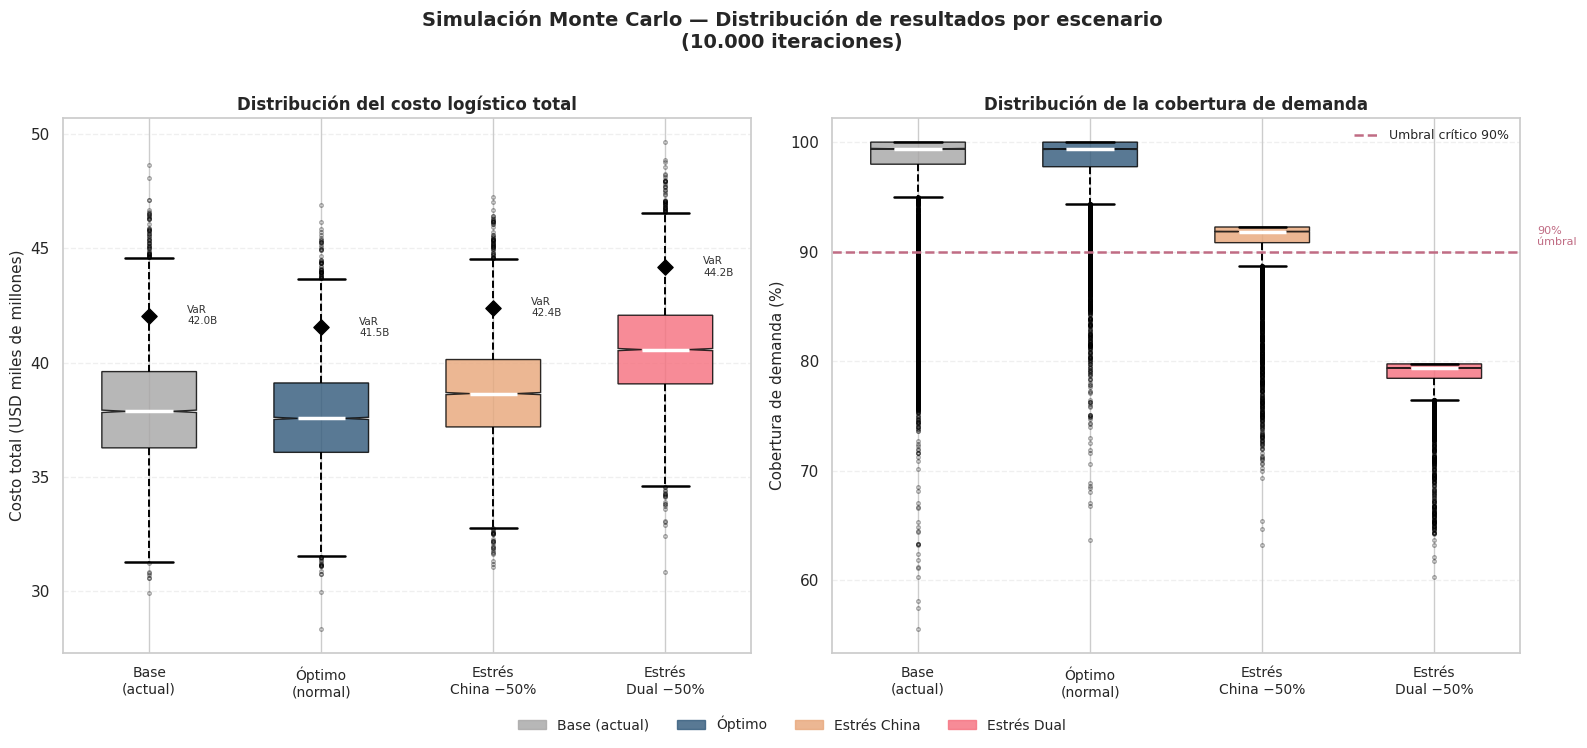
\includegraphics[width=0.98\textwidth]{resultados_distribucion_montecarlo.png}
\caption{\textbf{Boxplots Monte Carlo por escenario.} (Izq.) Costo total; diamantes negros = VaR 95\%: Base \$42.0B, Óptimo \$41.5B, Estrés China \$42.4B, Estrés Dual \$44.2B. (Der.) Cobertura; línea roja = umbral 90\%. \textbf{Observación clave:} bajo estrés China, Base completo bajo 90\%; Óptimo mayoritariamente arriba. Bajo estrés dual, ambos caen $\Rightarrow$ límite estructural.}
\label{fig:mc_boxplots}
\end{figure}

\vspace{-0.3cm}
\begin{table}[H]
\centering\caption{Resultados Monte Carlo: comparación simétrica Base vs. Óptimo (misma semilla)}\label{tab:montecarlo}
\footnotesize
\begin{tabular}{llcccc}
\toprule
\textbf{Escenario} & \textbf{KPI} & \textbf{Base} & \textbf{Óptimo} & \textbf{Mejora} \\
\midrule
\multirow{3}{*}{Normal}
  & VaR 95\% (USD M)       & 42.050  & 41.539  & \textcolor{verdeclaro}{$-1.2\%$} \\
  & Cobertura media        & 97.0\%  & 97.7\%  & \textcolor{verdeclaro}{$+0.6$ p.p.} \\
  & P(cob $<$ 90\%)        & 11.6\%  & 7.6\%   & \textcolor{verdeclaro}{$-4.0$ p.p.} \\
\midrule
\multirow{3}{*}{Estrés China $-50\%$}
  & VaR 95\% (USD M)       & 43.705  & 42.404  & \textcolor{verdeclaro}{$-3.0\%$} \\
  & Cobertura media        & 83.7\%  & 90.8\%  & \textcolor{verdeclaro}{$+7.1$ p.p.} \\
  & \textbf{P(cob $<$ 90\%)} & \textbf{100.0\%} & \textbf{15.0\%} & \textcolor{verdeclaro}{\textbf{$-85.0$ p.p.}} \\
\midrule
\multirow{3}{*}{Estrés dual (China+EE.UU.)}
  & VaR 95\% (USD M)       & 45.717  & 44.180  & \textcolor{verdeclaro}{$-3.4\%$} \\
  & Cobertura media        & 70.3\%  & 78.7\%  & \textcolor{verdeclaro}{$+8.4$ p.p.} \\
  & P(cob $<$ 90\%)        & 100.0\% & 100.0\% & \textcolor{rojosuave}{$0$ (límite estructural)} \\
\bottomrule
\end{tabular}
\end{table}

\vspace{-0.3cm}
\begin{hallazgo}
\textbf{Hallazgo 3 --- El valor de diversificar se revela en las colas.} Bajo condiciones normales, la mejora del óptimo es marginal ($-1.2\%$ en VaR). Bajo estrés severo de China, la probabilidad de falla crítica cae del \textbf{100.0\% al 15.0\%}: reducción de \textbf{85 puntos porcentuales}. La diversificación funciona como un seguro: no se aprecia en el día a día, pero salva la operación en eventos extremos.
\end{hallazgo}

% ==========================================================================
\section{Discusión}
% ==========================================================================

\subsection{Integración cualitativa-cuantitativa}

El valor diferencial del proyecto radica en cómo cada técnica habilita a las siguientes: (i) el AHP \emph{ancla cualitativamente} la decisión de diseño clave del LP (incluir $R_{max}$ como restricción dura), validada con CR=0.0074; (ii) el clustering K-Means \emph{focaliza} el problema en el Cluster 0 (89.6\% del valor), evitando diluir el análisis entre 189 países marginales; (iii) el LP \emph{explota} la estructura matemática del trade-off costo-riesgo; (iv) la sensibilidad dual \emph{cuantifica} el costo marginal de cada restricción; (v) el análisis de escenarios de política \emph{compara} tres posturas alternativas de $R_{max}$; (vi) Monte Carlo \emph{valida} la robustez del óptimo ante incertidumbre realista.

\subsection{Tres insights estratégicos}

\textbf{(1) La concentración es un riesgo latente invisible en promedios.} La mejora del $-1.2\%$ en VaR bajo condiciones normales podría llevar al decisor a concluir ``no vale la pena diversificar''. Monte Carlo bajo estrés demuestra lo contrario: el beneficio está en las colas, en los eventos extremos que los promedios ocultan.

\textbf{(2) La inercia comercial genera ineficiencia.} El hallazgo contraintuitivo más importante es que el portafolio óptimo tiene costo logístico \emph{recurrente} inferior al actual. La concentración en China no es resultado de optimización económica, sino de inercia histórica. Francia ---alternativa dominante (más barata \emph{y} más segura)--- simplemente no se había explotado.

\textbf{(3) Todo modelo tiene un límite estructural.} El estrés dual (China + EE.UU. $-$50\%) es inabsorbible por el Cluster 0 aisladamente. No es una falla del modelo, sino una guía honesta: la solución a ese escenario extremo está fuera del cluster, en el desarrollo del \emph{Cluster 1} (Proveedores Eficientes de Nicho: Suiza, Reino Unido, Irlanda) como segunda línea de suministro.

\subsection{Limitaciones}

(i) Dataset de 7 meses limita el análisis de estacionalidad. (ii) Juicios AHP construidos por el equipo con base en literatura; no validados con panel de expertos en comercio exterior colombiano. (iii) Scores $r_i$ calibrados con Global Risk Index (WEF, 2024) y Economic Complexity Index (Harvard); son estimaciones informadas, no mediciones empíricas de interrupciones históricas. (iv) Parámetros Monte Carlo (probabilidades, magnitudes) son supuestos razonables, no calibración sobre series históricas colombianas. (v) Modelo estático; una versión dinámica multi-periodo con decisiones de inventario sería extensión natural.

% ==========================================================================
\section{Conclusiones y Recomendación Final}
% ==========================================================================

\subsection{Hallazgos principales}

\begin{enumerate}[leftmargin=1.2em, itemsep=0.02em, topsep=0pt]
\footnotesize
\item \textbf{Concentración estructural confirmada:} HHI global=1.397 (no concentrado pero cercano al umbral); HHI del cluster=1.790 (moderadamente concentrado); Gini=0.916; $N_{eff}\approx 7.2$. China+EE.UU.=51\% del CIF. Estable mes a mes.
\item \textbf{AHP consistente (CR=0.0074):} diversificación (40.3\%) domina sobre costo (24.4\%). Este resultado cualitativo justifica incluir $R_{max}$ como restricción dura en el LP.
\item \textbf{K-Means focaliza la intervención:} Cluster 0 concentra 89.6\% del valor. El modelo opera sobre 23 países internacionales (excl. Colombia ZF).
\item \textbf{LP reduce concentración sin incrementar costo logístico recurrente:} HHI $-25.4\%$, riesgo $-15\%$, costo logístico $-0.53\%$; costo total F.O. $+1.02\%$ (componente único de transición). Mejora multicriterio simultánea.
\item \textbf{Sensibilidad dual:} 25 de 26 restricciones activas; $\pi_{R3}=-0.0112$; punto de inflexión paramétrico en $R_{max}\approx 3.69$.
\item \textbf{Análisis de escenarios de política:} Moderado ofrece HHI mínimo; Permisivo menor costo total; Estricto muestra trade-off desfavorable.
\item \textbf{Monte Carlo valida robustez:} P(cob$<$90\%) bajo estrés China cae de 100.0\% a 15.0\%. El estrés dual revela el límite estructural del Cluster 0.
\end{enumerate}

\subsection{Recomendación final}

\begin{recomendacion}
\textbf{Adoptar el escenario Moderado} ($R_{max}=0.85\cdot R_{actual}$) con estas cinco líneas de acción:
\begin{enumerate}[leftmargin=1.3em, itemsep=0.02em, topsep=0pt]
\footnotesize
\item \textbf{Redistribución gradual en 12--18 meses:} China $30\%\to 15.5\%$; Francia $1.5\%\to 18.6\%$; EE.UU. al techo 25\%. Horizonte extendido para absorber el costo único de transición sin choque operativo.
\item \textbf{Desarrollo activo del Cluster 1} (Suiza, Reino Unido, Irlanda, Suecia) como \emph{segunda línea de suministro}. El Monte Carlo bajo estrés dual demuestra que esta inversión es imprescindible.
\item \textbf{Contratos marco} con proveedores alternativos que reduzcan el $\tau$ efectivo ante señales tempranas de disrupción (habilitan sustitución rápida).
\item \textbf{Monitoreo trimestral:} HHI del cluster, riesgo ponderado y cobertura simulada. Reactivar el modelo LP si el HHI supera 1.500 o el riesgo ponderado supera $R_{actual}$.
\item \textbf{No reducir $R_{max}$ por debajo de 3.69} sin justificación estratégica específica: bajo ese umbral, el costo marginal de reducir riesgo crece aceleradamente según el análisis paramétrico.
\end{enumerate}
\end{recomendacion}

\vspace{-0.1cm}
\subsection*{Referencias}
\footnotesize
\begin{itemize}
    \item Charnes, A., \& Cooper, W. W. (1961). \textit{Management models and industrial applications of linear programming} (Vols. 1--2). Wiley.

    \item Chopra, S., \& Sodhi, M. S. (2014). Reducing the risk of supply chain disruptions. \textit{MIT Sloan Management Review}, 55(3), 73--80.

    \item Christopher, M., \& Peck, H. (2004). Building the resilient supply chain. \textit{The International Journal of Logistics Management}, 15(2), 1--14. \url{https://doi.org/10.1108/09574090410700275}

    \item Datos Abiertos Bogotá. (s. f.). \textit{Plataforma Distrital de Datos Abiertos de Bogotá}. Recuperado el 23 de abril de 2026, de \url{https://datosabiertos.bogota.gov.co/}

    \item Hausmann, R., \& Hidalgo, C. A. (Eds.). (2014). \textit{The atlas of economic complexity: Mapping paths to prosperity}. MIT Press.

    \item Manuj, I., \& Mentzer, J. T. (2008). Global supply chain risk management strategies. \textit{International Journal of Physical Distribution \& Logistics Management}, 38(3), 192--223. \url{https://doi.org/10.1108/09600030810866986}

    \item Saaty, T. L. (1980). \textit{The analytic hierarchy process: Planning, priority setting, resource allocation}. McGraw-Hill.

    \item Simchi-Levi, D., Schmidt, W., \& Wei, Y. (2014). From superstorms to factory fires: Managing unpredictable supply-chain disruptions. \textit{Harvard Business Review}, 92(1--2), 96--101. \url{https://hbr.org/2014/01/from-superstorms-to-factory-fires-managing-unpredictable-supply-chain-disruptions}

    \item U.S. Department of Justice, \& Federal Trade Commission. (2023). \textit{Merger guidelines}. \url{https://www.justice.gov/d9/2023-12/2023\%20Merger\%20Guidelines.pdf}

    \item World Economic Forum. (2024). \textit{The global risks report 2024}. \url{https://www.weforum.org/publications/global-risks-report-2024/}
\end{itemize}

\end{document}
